\chapter{Crittografia Simmetrica}
Nella struttura di un cifrario simmetrico si possono individuare due distinte componenti. Il primo è l'\textbf{algoritmo}, o semplicemente l'insieme di operazioni che applicano una determinata \textbf{permutazione} ad una porzione di \textit{plain text}. Il termine ``porzione'' è definito ad una caratteristica del cifrario. Infatti può essere una \textit{singola lettera}, un \textit{gruppo di lettere} o (come nei cifrari moderni) un \textit{gruppo di bit} detto comunemente \textbf{blocco}. Una \textbf{permutazione} di un insieme di \textit{n} oggetti è uno dei possibili modi in cui gli \textit{n} oggetti si possono disporre linearmente; cioè è uno dei possibili ordinamenti degli oggetti. In termini matematici, una permutazione di un insieme \textit{I} è una funzione invertibile in \textit{I} stesso. Si noti che l'ovvio requisito di invertibilità delle cifratura, che si precisa fondamentalmente con l'invertibilità delle permutazioni, in termini pratici implica che il plaintext e ciphertext abbiamo sempre la \textbf{stessa lunghezza}. La seconda componente di un algoritmo è il \textbf{mode of operation} ovvero come le ``porzioni'' di plaintext vengono opportunamente concatenate una con l'altra.
\newline
Quelli appena descritti sono però definiti \textbf{cifrari a blocchi}. Esistono in letteratura cifrari che considerano il messaggio come \textit{flusso continuo} di bit e che utilizzano la chiave per generare un corrispondente flusso di bit, nota come \textbf{round key} che verrà posta in XOR con i bit del messaggio. Tali cifrari sono noti come \textbf{\textit{stram cipher}}, vengono normalmente utilizzati nelle comunicazione telefonoiche, ad esempio.

\section{Cifrari Classici: Cesare e Vigenère}
Considerando i messaggi scritti in un generico alfabeto $\Sigma$ e consideriamo un \textbf{ordinamento circolare} dei caratteri, ovvero che il primo è il successore dell'ultimo. Nel \textbf{Cifrario di Cesare} la cifratura avviene:
\begin{enumerate}
    \item Viene applicata una \textbf{permutazione} ad ogni carattere del messaggio che consiste in uno \textbf{shift} (slittamento) di \textit{k} posizioni in avanti.
    \item In questo modo ogni carattere \textit{x} del plaintext viene sostituito con il carattere \textit{x + k} rispetto all'ordinamento circolare di $\Sigma$.
    \item In questo caso il \textbf{mode of operation} è applicare la stessa permutazione ad ogni carattere.
\end{enumerate}
In questo caso la \textbf{chiave privata} non è altro che \textit{k}, ovvero il valore dello slittamento. In questo tipo di cifrario la \textbf{decifrazione} non è altro che uno \textbf{shift} di \textit{k} posizione di ogni carattere del ciphertext all'indietro. Considerando un carattere del ciphertext \textit{x'} avremo che \textit{x = x' - k} per ogni carattere del ciphertext. Possiamo anche dire che se la chiave di cifratura è \textit{k} allora la chiave di decifrazione è \textit{-k} ovvero il suo opposto. In questo semplice cifrario il \textbf{numero di chiavi}, che coincide con il numero di possibili slittamenti, è limitato dalla cardinalità dell'alfabeto.
\newline
Prendiamo ora in considerazione ora un esempio di crittoanalisi per il cifrario di Cesare. Consideriamo l'alfabeto \textbf{\textit{$\Sigma$ = \{a, b, .., z\} $\cup$ \{.\} $\cup$ \{,\} $\cup$ \{'\}}} e considerando come \textbf{cipher = \textit{kdcxiitzz,ev,yhtjeved,bv,yhth,ew,vxithx}} potremmo utilizzare una procedura di crittoanalisi di \textbf{brute force} (forza bruta) ovvero tentare per tutti i possibili valori di \textit{k} quello cha ha per risultato un testo sensata. Considerando il codice~\ref{lst:ceaser-bruteforce} possiamo andare ad iterare su tutti i possibili valori di \textit{k} e farci stampare a video il risultato di ogni iterazione in questo modo è possibile andare a leggere tutte le possibili permutazioni di \textit{x} e andare a decifrare il contenuto del messaggio. 
\newline
Possiamo notare che per \textit{k = 19} si può leggere il messaggio \textit{unmessaggiocifratoconilcifrariodicesare} che interpretandolo correttamente diviene \textit{un messaggio cifrato con il cifrario di cesare}, il fatto di rimuovere gli spazi serve per evitare di dare al crittoanalista un'informazione, ovvero la lunghezza di ogni parola.

\begin{lstlisting}[label=lst:ceaser-bruteforce, basicstyle=\small]
    alphabet = "abcdefghijklmnopqrstuvwxyz.,'"

    def decrypt(cyphertext, key):
        n = len(alphabet)
        cyphertext = ''.join([alphabet[(alphabet.find(c) + key) % n] for c in plaintext])

    unknowntext = "kdcxiitzz,ev,yhtjeved,bv,yhth,ew,vxithx"
    for k in range(len(alphabet)):
        print(f"{k}\t{decrypt(unknowntext, -k)}")
    
    # output
    19	unmessaggiocifratoconilcifrariodicesare
\end{lstlisting}

Il \textbf{cifrario di Cesare} è forse il più semplice caso di \textbf{cifrario mono-alfabetico} infatti utilizza una sostituzione fissa per ogni carattere, in altri termini, fissato l'alfabeto di riferimento $\Sigma$, un \textit{cifrario mono-alfabetico} è definito da una \textbf{singola permutazione} ripetuta per tutti i caratteri. Un'altra caratteristica del cifrario di cesare è che la \textbf{permutazione} è una semplice \textbf{rotazione} e per riuscire a rompere questo cifrario è necessario la conoscenza di un singolo numero intero, compreso fra 0 e la cardinalità dell'alfabeto. La chiave è l'unica \textbf{informazione segreta} di un cifrario mono-alfabetico e quindi il testo cifrato deve dipendere sempre dalla permutazione. A chiavi diverse bisogna che ci siano diversi ciphertext, in caso contrario per un attaccante ci sarebbero meno chiavi distinte da provare e questo potrebbe agevolare gli attacchi. La permutazione deve apparire il più possibile casuale. Questo garantisce che la conoscenza di come viene mappata una lettera (o un gruppo di bit) non fornisce alcuna conoscenza sulla mappatura delle altre. 

\newpage
Noto il fatto che per calcolare le possibili permutazioni di una certa lunghezza l'operazione è il fattoriale avremo un numero di permutazione tali a: $n_p = card(\Sigma)!$

\begin{lstlisting}[label=lst:n-perm, basicstyle=\small]
    alphabet = "abcdefghijklmnopqrstuvwxyz .,'"
    print(factorial(len(alphabet)))

    # output
    265252859812191058636308480000000
\end{lstlisting}

\textbf{Crittoanalisi}: per un generico cifrario mono-alfabetico il numero di possibili chiavi è dunque pari al numero di permutazioni dell'insieme dei caratteri dell'alfabeto, in questo caso un attacco \textit{brute force} è impensabile, nel caso di cifrari mono-alfabetici la crittoanalisi più efficace è quella bata sull'\textbf{analisi delle frequenze}. L'attacco si basato sull'ipotesi che la frequenza con cui compaiono i singoli caratteri nel plaintext sia conforme alla più generale \textbf{frequenza nella lingua} con cui il testo è scritto, questo mette come vincolo il fatto di conoscere la lingua del testo cifrato che si vuole decodificare e l'ipotesi sarà tanto più verificata quanto più il plaintext è lungo. Un'altro vincolo è quello di disporre di una \textbf{stima delle frenquenze dei caratteri} in quella lingua.
\\ \newline
\textbf{Vigenère: un cifrario poli-alfabetico}, ovvero che uno stesso carattere non è sempre soggetto alla stessa trasformazione. Le chiavi sono \textbf{sequenze di caratteri dell'alfabeto $\Sigma$}, ciascuno dei quali deve essere interpretato come il numero corrispondente alla sua \textbf{posizione nell'alfabeto} (partendo da 0). Ad esempio se il palintext fosse \textbf{algorithms} e la chiave fosse \textbf{crypto}, il ciphertext verrebbe determinato in questo modo:
\begin{center}
    \begin{math}
        \begin{array}{rcccccccccc}
            \textrm{key}:&\mathtt{c}&\mathtt{r}&\mathtt{y}&\mathtt{p}&\mathtt{t}&\mathtt{o}&\mathtt{c}&\mathtt{r}&\mathtt{y}&\mathtt{p}\\
            \textrm{$key_i$}:&\mathtt{2}&\mathtt{17}&\mathtt{24}&\mathtt{15}&\mathtt{19}&\mathtt{14}&\mathtt{2}&\mathtt{17}&\mathtt{24}&\mathtt{15}\\
            \textrm{plaintext}:&\mathtt{a}&\mathtt{l}&\mathtt{g}&\mathtt{o}&\mathtt{r}&\mathtt{i}&\mathtt{t}&\mathtt{h}&\mathtt{m}&\mathtt{s}\\
            \textrm{$plaintext_i$}:&\mathtt{0}&\mathtt{11}&\mathtt{6}&\mathtt{14}&\mathtt{17}&\mathtt{8}&\mathtt{19}&\mathtt{7}&\mathtt{12}&\mathtt{18}\\
            \textrm{ciphertext}:&\mathtt{c}&\mathtt{c}&\mathtt{e}&\mathtt{d}&\mathtt{k}&\mathtt{w}&\mathtt{v}&\mathtt{y}&\mathtt{k}&\mathtt{h}\\
            \textrm{$ciphertext_i$}:&\mathtt{2}&\mathtt{2}&\mathtt{4}&\mathtt{3}&\mathtt{10}&\mathtt{22}&\mathtt{21}&\mathtt{24}&\mathtt{10}&\mathtt{7}
        \end{array}
    \end{math}
\end{center}

Avremo quindi una funzione di encryption del tipo:
\begin{lstlisting}[label=lst:enc-vigenere, basicstyle=\small]
    alphabet = "abcdefghijklmnopqrstuvwxyz"
    plain, key = "algorithms", "crypto"

    a = {alphabet[i]: i for i in range(len(alphabet))}
    b = {i: alphabet[i] for i in range(len(alphabet))}

    def encryption(plain, key):
        cipher = ""
        for i in range(len(plain)):
            x = a.get(plain[i])
            k = a.get(key[i % len(key)])
            
            cipher += b.get((x + k) % len(alphabet))
        return cipher

        print(f"[ PLAIN ]: {plain}, [ CIPHER ]: {encryption(plain, key)}")

    # output
    [ PLAIN ]: algorithms, [ CIPHER ]: ccedkwvykh
\end{lstlisting}

Per la \textbf{decifrazione} si procede allo stesso modo utilizzando però, sempre con la stessa chiave, il valore di slittamento all'indietro.
\\ \newline
\textbf{Attacchi al cifrario di Vigenère}: senza l'ausilio di un computer questo tipo di cifrario era praticamente inattaccabile, soprattuto con una chiave casuale, tutt'oggi è difficilmente attaccabile in caso di chaive casuale con lunghezza confrantabile con il testo e non riutilizzata più volte. In quest'ultimo caso, il cifrario ``degenera'' infatti in una sorta di \textbf{one-time pad testuale} noto anche come \textbf{\textit{cifrario di Vernam}}. Nel caso in cui invere la chiave è relativamente corta rispetto al testo è possibile effettuare un attacco la cui prima parte è quella di indentificare la \textbf{lunghezza della chiave}.
\newline
Consideriamo, come esempio, un testo cifrato \textbf{C = \textit{fxbxzktwrdvfcsfxbxqwplbn}} e notiamo che la sequenza di 4 caratteri \textbf{fxbx} si ripete ad una distanza di 14 posizioni. Potremo quindi iniziare a fare dei check sulle possibilità di crittoanalisi per questo ciphertext.
\\ \newline
\resizebox{\textwidth}{!}{%
\begin{forest}
  for tree={
    child anchor=west,
    parent anchor=east,
    grow'=east,
  %minimum size=1cm,%new possibility
  text width=4cm,%
    draw,
    anchor=west,
    edge path={
      \noexpand\path[\forestoption{edge}]
        (.child anchor) -| +(-5pt,0) -- +(-5pt,0) |-
        (!u.parent anchor)\forestoption{edge label};
    },
  }
    [\textbf{Testo Cifrato con Ripetizioni}
        [Testo uguale - Chiave Uguale
            [ La chiave è più lunga ma il testo è ripetuto ]
            [La chiave è più corta: allora è un divisore del numero dei caratteri che si interpone tra le due ripetizioni
                [\textbf{Attacco al Cifrario di Vigenère}]
            ]
        ]
        [Testo Diverso - Chiave Diversa
            [ Combinazione che da il risultato uguale]
        ]
    ]
\end{forest}
}%

Una volta che ipotizziamo di essere nella casistica corretta per effettuare un attacco di crittografia, \textit{Eve} può provare ad indovinare la lunghezza della chiave, che può essere un divisore di 14: 2, 7, 14. Considerando 2 come chiave troppo corta e 14 come chiave troppo lunga, proviamo a portare avanti l'attacco considerando la chiave lungha 7 caratteri. A questo punto \textit{Eve} può tentare almeno tre strade:
\begin{enumerate}
    \item \textbf{Attacco brute force}: computazionalmente non troppo oneroso, infatti le chiavi possibili sono soltanto $26^7 = 8031810176$.
    \item \textbf{Analisi delle frequenze}: se il testo è abbastanza lungo si può provare a stimare le frequenze considerando che due identici caratteri del testo cifrato corrispondono con certezza allo stesso carattere del plaintext se e solo se la loro posizione differisce di un multiplo di 7.
    \item \textbf{Attacco a Dizionario}: ipotizzando che la chiave non sia casuale, \textit{Eve} può provare tutte le parole di 7 lettere di un dizionario (della lingua da cui proviene il plaintext).
\end{enumerate}

\newpage
\section{One-time pad - Cifrario di Vernam}

Il \textbf{One-time pad} è ``teoricamente'' il cifrario che ha una \textbf{sicurezza incondizionata} ovvero il testo cifrato generato non contiene abbastanza informazioni per determinare il testo in chiaro, indipendentemente da quanto testo cifrato sia disponibile, è computazionalmente molto oneroso per essere utilizzato. Il funzionamento consiste nel prendere un messaggio (plaintext) \textbf{\textit{P}}, ovvero una \textit{string di bit}, e una chiave che è una sequenza di bit della \textit{stessa lunghezza del testo in chiaro}. Avremo quindi che:
\begin{center}
    $c_i = p_i\oplus k_i,\qquad i=0,1,\ldots,|P|-1$
\end{center}
Ovvero che il testo cifrato, ciphertext, sarà lo \textit{xor} bit a bit tra il plaintext e la chiave. 
\newline
Affinché la chiave sia adatta bisogna che rispetti una serie di condizioni:
\begin{itemize}
    \item Ogni bit della chiave deve avere valore 0 oppure 1 con \textbf{uguale probabilità} e in modo \textbf{indipendente} dal valore dei bit precedenti, ovvero: 
    \begin{center}
        $prob[k_i=0]=prob[k_i=1]=\frac{1}{2}\quad$
        \\
        $prob[k_i=v|k_{i-1}=w]=prob[k_i=v],\,\,v,w\in\{0,1\}$
    \end{center}
    \item La chiave deve essere \textbf{utilizzata una sola volta}, è quindi necessario generare una nuova chiave ogni volta che si vuole inviare un messaggio.
\end{itemize}
\'{E} quindi possibile osservare che per i bit del messaggio cifrato valgono le stesso proprietà, indipendentemente da come sono scelti i bit del messaggio ovvero del plaintext.
\newline
La \textbf{sicurezza del one-time pad} deriva dal fatto che se la chiave è stata scelta come indicato sopra ed è di lunghezza \textit{n} (quindi \textit{n} sarà anche la lunghezza di \textit{P}) ogni messaggio ha una possibiltà pari $2^{-n}$ di essere decriptato. Nel caso in cui due messaggi in chiaro \textit{$P_1$}  e \textit{$P_2$} vengono cifrati con la stessa chiave \textit{K} allora è possibilie ottenere della conoscenza sulla comunicazione. 
\begin{center}
    \begin{eqnarray*}
        C_1\oplus C_2&=&(P_1\oplus K)\oplus(P_2\oplus K)\\
                    &=&(P_1\oplus P_2)\oplus(K\oplus K)\\
                    &=&(P_1\oplus P_2)\oplus O\\
                    &=&P_1\oplus P_2
    \end{eqnarray*}
\end{center}
In quyesto modo l'attaccante viene a conoscenza dello \textbf{xor dei due messaggi} e dunque, conoscendone uno dei due (o parte di uno dei due) verrebbe a conoscenza anche (parte de)l'altro.

\section{Obiettivi generali di sicurezza}
Esistono più obiettivi di un attacco da parte di \textit{Eve}, di cui ``capire il messaggio'' non è neppure il più estremo, potrebbe essere che voglia \textbf{determinare la chiave} che permetterebbe di mettere in chiaro uno o più messaggi o un altro consiste nel far passare per autentico un messaggio che invece \textit{Eve} ha \textbf{alterato} o prodoto nella sua interezza. \'{E} quindi necessario distinguere i due principali obiettivi:
\begin{itemize}
    \item \textbf{\textit{Indistinguibilità}}: è la proprietà di uno schema di cifratura i cui testi cifrati per un attaccante sono essenzialmente \textit{indistinguibili} da stringhe di bit generate casualmente. Facciamo un esempio: \textit{Alice} e \textit{Eve} sono gli attori, \textit{Eve} produce \textbf{due messaggi in chiaro} e li sottopone ad \textit{Alice}, che deciderà, a caso e con uguale probabilità, quale dei due cifrare, e presenterà quello cifrato ad \textit{Eve}, il cifrario è indistinguibile se \textit{Eve} non riesce ad indovinare quale messaggio sia stato cifrato con probabilità significativamente maggiore di $\frac{1}{2}$.
    \item \textbf{\textit{Non malleabilità}}: ovvero se, dato un ciphertext \textit{$C_1$} corrispondente ad un plaintext \textit{$P_1$}, risulta impossibile per \textit{Eve} creare un secondo ciphertext \textit{$C_2$} corrispondente ad un plaintext \textit{$P_2$} che abbia una qualche relazione con \textit{$P_1$}. La non malleabilità è una proprietà che ha a che fare con l'\textbf{integrità} dei messaggi.
\end{itemize}
Nel caso del \textit{one-time pad} si può affermare che è soa indistinguibile che non malleabile a meno che una stessa chiave venga utilizzata per due o più plaintext diversi.

\newpage
\section{Cifrari a Blocchi}
I cifrari a blocchi moderni vengono definiti a blocchi in quanto lavorano su blocchi di lunghezza fissa, indichiamo con \textit{B} il numero di bit di un blocco, che normalmente è compreso nell'intervallo tra i 64 bit e i 256 bit. Nel caso in cui il plaintext da cifrare abbia una lunghezza superiore rispetto a \textit{B} allora il plaintext verrà diviso in blocchi con lunghezza pari a \textit{B}, ma nel caso in cui l'ultimo blocco o l'ìntero plaintext abbia lunghezza inferiore a \textit{B} verranno aggiunti \textbf{bit di padding} (riempimento). Nel caso in cui il plaintext venga diviso in sottoblocchi che verranno cifrati separatamente sarà necessario uno schema di concatenazione di vari blocchi, questo è identificato come \textbf{mode of operation}.
\newline
Sia padding che mode of operation sono tutt'altro che banali utilizzando schemi obsoleti o ``sbagliati'' nella circostanza di criptazione dare vantaggi ai crittoanalisti per la decifrazione malevola del crittogramma.
\newline
\'{E} quindi necessario scegliere correttamente non solo il mode of operation e lo standard di padding che si vuole adottare ma anche considerare la lunghezza di \textit{B} in quanto bisogna trovare un valore per cui \textit{B} non sia troppo lungo con lo scopo di incrementare l'efficienza (\textbf{hardware dedicato}), ma non deve essere neanche troppo corto per evitare problemi legati alla sicurezza ma anche ridurre l'overhead legato al trattamento di molti messaggi corti. Nel caso in cui un blocco sia lungo \textit{B} piccolo, un attaccante potrebbe precompilare una tabella $2^\textit{B}$ posizioni in cui alla generica posizione \textit{i} è memorizzato il plaintext che ha \textit{i} come ciphertext
\\ \newline
\textbf{\textit{Codebook Attack}}: nel caso di \textit{B} piccolo corrisponderebbe ad un semplice \textbf{table lookup}, altre tipologie di attacco che invece potrebbero utilizzare ad esempio, il tempo di esecuzioni di operazioni su chiave privata vengono chiamati \textbf{\textit{Side Channel Attack}}.
\\ \newline
Possiamo andare a descrivere in maniera astratta uno \textbf{\textit{Schema di Block Cipher}}: andiamo a definire che una chiave \textit{k} necessaria sia per la cifrazione che decifrazione ha normalmente una lunghezza compresa tra \textbf{128 e 256 bit}, e abbiamo assimilato che la cifratura non è altro che una \textbf{permutazione} poiché plaintext e ciphertext sono formati dallo stesso numero di bit. \'{E} anche noto che ad ogni plaintext di \textit{B} bit deve corrispondere \textbf{un unico} ciphertext di \textit{B} bit, e viceversa, altrimenti il processo non sarebbe invertibile. Potremmo visualizzare la cifratura come un processo di \textbf{due fasi}:
\begin{itemize}
    \item data la chiave \textit{k}, si seleziona una specifica \textbf{\textit{Lookup Table $T_k$}}, di $2^\textit{B}$ posizioni, che memorizza una specifica permutazione delle sequenze di \textit{B} bit.
    \item la cifratura corrisponde ad un accesso a $T_k$ usando il plaintext come chiave su quella tabella e riuscendo a recuperare il ciphertext.
\end{itemize}
\'{E} immediato osservare che la lunghezza della chiave \textit{k} determini il \textbf{numero delle lookup table} e dunque di permutazioni, che possono essere utilizzate in un cifrario a blocchi con chiavi di quella lunghezza. Se dunque la chiave è lungha \textit{m} bit, allora il numero di permutazioni usabili è $2^m$. Questo valore è apparentemente grande infatti considerando che le permutazioni totali di \textit{B} bit, che cresce in maniera molto più repentina ovvero: $2^B!$. Sono presenti però delle permutazioni di \textit{B} bit che però vengono scartate, ovvero quelle che possono essere espresse \textbf{mediante trasformazioni lineari affini invertibili} sul campo $Z_2$.
\begin{center}
    \begin{math}
        xP + b = y(x)
    \end{math}
\end{center}
in cui \textit{P} è una matrice non singolare di ordine \textit{B} su $Z_2$ mentre \textit{x} (il plaintext), b e $y(x)$ (il ciphertext) sono vettori riga di \textit{B} element, sempre con elementi in $Z_2$.
\\ \newline
Un cifrario a blocchi ha come scopo, alla fine, quello di \textbf{forzare la non-linearità} della permutazione realizzato tramite i concetti di:
\begin{itemize}
    \item \textbf{\textit{Diffusione}}: ogni minima modifica localizzata in un punto del plaintext, si rifletta su tutto il ciphertext.
    \item \textbf{\textit{Confusione}}: è la caratteristica che \textbf{distrugge ogni regolarità}, ogni eventuale pattern nel plaintext.
\end{itemize}

\subsection{Feistel Network}
La rete di Feistel non è un vero e proprio cifrario a blocchi, ma si tratta di uno schema per realizzare cifrari a blocchi, fra i quali è presente \textbf{Digital Encryption Standard} (\textbf{\textit{DES}}) che rimase per molti anni lo standard per la cifratura simmetrica, ora deprecato e sostituito da \textbf{Advanced Encryption Standard} (\textbf{\textit{AES}}). La rete di Feistel unisce i concetti di cifrario prodotto a quelli di Shannon, ovvero \textit{diffusione} e \textit{confusione}, riuscendo ad approssimare il funzionamento di un cifrario a blocchi ideale attraverso:
\begin{itemize}
    \item l'alterazione di tecniche di \textbf{sostituzione} a quelle di \textbf{permutazione} per la confusione dei bit.
    \item \textbf{chiave} a \textit{k} bit per un blocco a \textit{n} bit ($2^k << 2^n$).
\end{itemize}
La rete di Feistel è composta da un certo numero di \textbf{stadi con identica struttura} noti anche come \textbf{round}. Ad ogni stadio viene utilizzata una specifica \textbf{round key $k_i$}, una diversa per ogni stadio sono tutte derivabili dalla \textbf{chiave generale}, questo avviene tramite un algoritmo (ovviamente reversibile) chiamato \textbf{key schedule}. Considerando la lunghezza di un blocco della rete di Feistel di \textit{B}, ad ogni stadio \textit{i} opera su due semiblocchi $L_i$ e $R_i$ ognuno di lunghezza $\frac{B}{2}$. Nella prima iterazione la concatenazione $L_0 || R_0$ dei semiblocchi è proprio il blocco iniziale da cifrare. Il blocco di destra $R_i$ passa inalterato come blocco di sinistra $L_{i+1}$, mentre il blocco di destra dell'iterazione successiva, $R_{i+1}$ è ottenuto applicando ad $R_i$ una trasformazione \textbf{\textit{F}} che dipende dalla round key e il cui risultato viene posto in xor bit a bit con il valore di $L_i$.

\begin{figure}[h]
    \centering

    \begin{minipage}[t]{0.3\textwidth}
        \centering
        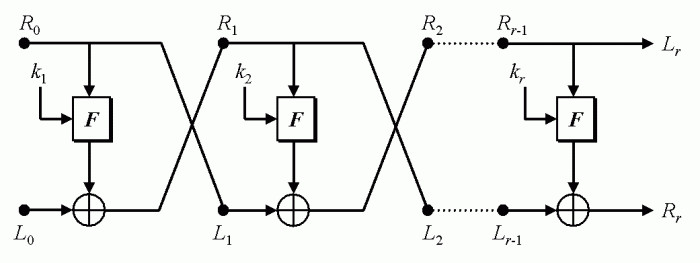
\includegraphics[width=\textwidth, valign=c]{feistel.jpg}
    \end{minipage}
    \hfill
    \begin{minipage}[t]{0.6\textwidth}
        \begin{math}
            \begin{cases}
                L_1 = R_0 \\
                R_1 = L_0 \oplus f(R_0, k_1)
            \end{cases}
            \cup
            \begin{cases}
                L_{i+1} = R_i \\
                R_{i+1} = L_i \oplus f(R_i, k_i)
            \end{cases}
        \end{math}
    \end{minipage}
\end{figure}

Il processo è \textbf{reversibile} viste le \textbf{proprietà dello xor esclusivo}, visivamente può essere eseguita ``rovesciando'' tutte le frecce e dunque la direzione input/output dei semiblocchi, ma \textbf{non} è necessario. Infatti è sufficente alimentare la stessa rete con input $R_r||L_r$ e naturalmente usando le round key in ordine inverso. Il numero di roun è legato alla diffusione.
\\ \newline
La \textbf{funzione \textit{F}} i cui metodi implementativi variano in base alla tipologia di cifrario scelto ha come scopo:
\begin{itemize}
    \item di inserire la \textit{chiave nel processo} ``mischiandola'' con i bit del messaggio.
    \item di assicurare \textit{dipendenza \textbf{non} lineare} fra plaintext e ciphertext, attraverso un \textbf{S-Box}.
\end{itemize}
Nel caso (ad esempio) di \textbf{DES} la funzione \textbf{\textit{F}} svolge i seguenti passaggi:
\begin{enumerate}
    \item i 32 bit di $R_i$ vengono espansi a 48 bit tramite la duplicazione di alcuni bit.
    \item l'output di questa computazione viene messo in \textbf{\textit{xor}} con la \textit{round key} che nel caso di \textbf{DES} è a 48 bit.
    \item il risultato deve essere riportato a 32 bit, in vista dello \textbf{\textit{xor}} finale con il semiblocco $L_i$, \textbf{S-Box}, che in realtà è costituita da 8 tabelle, ciascuna indicizzata da 6 bit e le cui posizioni contengono 4 bit di output.
    \item il risultato prodotto dall'S-Box $\Rightarrow$ $4 (bit) * 8 (tabelle)$ viene permutato e posto in \textbf{\textit{xor}} con il semiblocco $L_i$ e quindi saremo pronti per l'iterazione successiva.
\end{enumerate}

\begin{figure}[h]
    \centering
    \begin{minipage}[t]{0.45\textwidth}
        \centering
        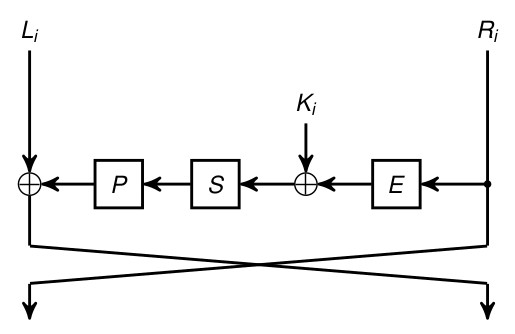
\includegraphics[width=\textwidth, valign=c]{desround.jpg}
        \caption{F function DES}
    \end{minipage}
    \hfill
    \begin{minipage}[t]{0.45\textwidth}
        \centering
        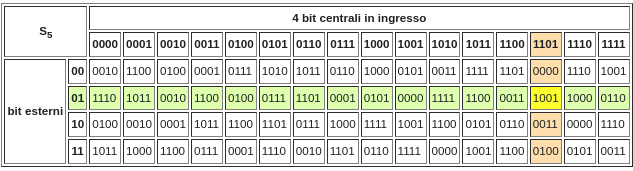
\includegraphics[width=\textwidth, valign=c]{sbox.png}
        \caption{DES S-Box}
    \end{minipage}
\end{figure}

Il \textbf{\textit{Key Schedule}} è l'algoritmo con cui, dalla chiave iniziale, vengono ottenute le varie \textbf{\textit{Round Key}}, considerando sempre il caso di \textbf{Digital Encryption Standard} osserviamo che presenta una \textit{key} di 56 bit con 8 bit di parità, che viene suddivisa in due metà da 28 bit ciascuna.
\newline
Ad ogni round, ciascuna metà viene \textbf{ruotata} a sinistra di 1 o 2 posizioni (a seconda del round), dopo di ché viene formata la \textbf{\textit{round key}} prelevando 24 bit da entrambe.

% \subsection{Digital Encryption Standard}

% \subsection{Advanced Encryption Standard}

\section{Mode of Operation}
Il \textit{mode of operation} è l'algoritmo che permette la cifratura complessiva di un messaggio utilizzando un cifrario a blocchi per le singole porzioni del messaggio. Inanzitutto viene eseguito un riempimento, anche noto come \textbf{\textit{padding}} del messaggio iniziale \textit{M} di modo che la sua lunghezza sia multiplo della dimensione dei blocchi del cifrario selezionato. Indicheremo con $P = P_1||P_2||...||P_n$ la suddivisione dei blocchi dopo il padding.

\subsection{Electronic Codebooks Mode - ECB}
È l'algoritmo più \textbf{semplice}, ma anche il più \textbf{vulnerabile}. Ogni singolo blocco viene cifrato in manierea \textit{indipendente}, ma attraverso una \textit{stessa chiave}: 
\begin{center}
    $C_i = E(P_i, k)\;\;\;i = 1, 2, .., n$
\end{center}
dove indicheremo con \textbf{\textit{E}} la funzione realizzata dal cifrario per cifrare il plaintext e \textit{k} la chiave privata. Il problema del \textbf{\textit{ECB}} è che a \textbf{blocchi di plaintext identici} corrispondono \textbf{blocchi di ciphertext identici}. Ovviamente la problematica è più di rilievo nel caso di immagini o grafici rispetto a messaggi, ad esempio:
\begin{figure}[h]
    \centering
    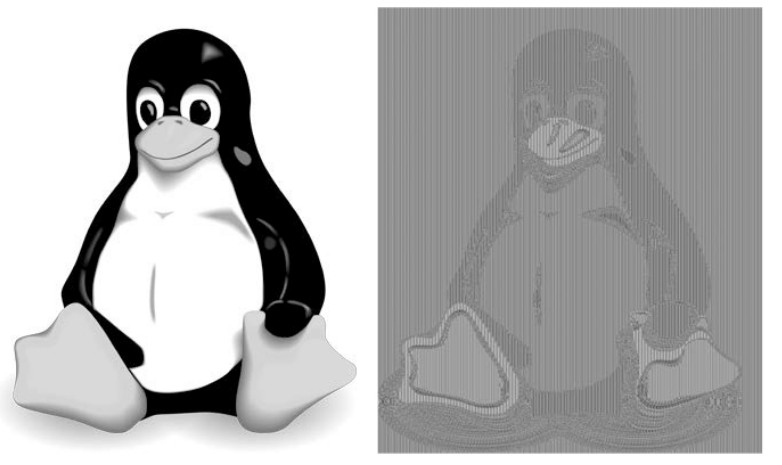
\includegraphics[width=0.5\textwidth, valign=c]{penguin.jpg}
    \caption{Source: J.P. Aumasson, Serious Cryptography, No Starch Press (2018)}
\end{figure}

\subsection{Cipher Block Chaining - CBC}
In questo differente \textit{mode of operation} la cifratura avviene nel seguente modo: 
\begin{center}
    \begin{math}
        \begin{cases}
            C_1 = E(P_1 \oplus IV, k) \\
            C_i = E(P_i \oplus C_{i-1}, k)\;\;\;i = 2, 3, ..., n
        \end{cases}
    \end{math}
\end{center}
dove \textbf{\textit{IV}} indica un blocco iniziale, \textbf{\textit{Initialization Vector}}. La decifrazione è possibile, grazie alle \textit{proprietà dello \textbf{xor} esclusivo}.
\begin{center}
    \begin{math}
        \begin{cases}
            P_1 = D(C_1, k) \oplus IV \\
            P_i = D(C_i, k) \oplus C_{i-1} \;\;\;i = 2, 3, ..., n
        \end{cases}
    \end{math}
\end{center}
Il \textit{vettore di inizializzazione} può essere scelto in vario modo ma la soluzione più comune è di utilizzare un \textbf{\textit{nonce}}.
\\ \newline
\textcolor{red}{\textbf{ATTENZIONE}}: è possibile effettuare un attacco di tipo \textbf{\textit{Padding Oracle}} se vengono soddisfatte le seguenti condizioni:
\begin{enumerate}
    \item Lo schema di \textbf{padding \textit{ISO/IEC 9797-1}} e con qualsiasi cifrario a blocchi che operi unitamente al \textbf{mode of operation \textit{CBC}}.
    \item \textit{Eve} deve poter effettuare \textbf{query di decifrazione} (quindi sarà unicamente necessario che \textit{Eve} conosca \textbf{un} ciphertext) ad un server che risponde e \textbf{sollevi un eccezione} in caso di \textbf{\textit{padding malformato}} 
\end{enumerate}